\chapter{Static Computational Optical Undersampled Tracker}\label{chap:Scout}

\section{Motivation for the Static Computational Undersampled Tracker}

In large-area persistent surveillance, traditional \gls{isomorphic} sensing systems which are based on the Shannon-Nyquist sampling theorem must acquire, process, store, and transmit large amounts of data to achieve high spatial and temporal resolution. These sensors are often on airborne or orbiting platforms so this often leads to a large \gls{swap-c}. However, if the application is specific to only tracking moving targets, the information content in the signal-of-interest is relatively low compared to the data in the measurement. Furthermore, in many situations the background is relatively static to field-of-view of the sensor, one can design a sensor to focus on temporally varying aspects of the target to promote \gls{sparsity}. This intuitively leads one to turn to techniques based on \gls{compressive sensing}. As I discussed in \Cref{chap:Introduction} and \Cref{chap:Formalism}, \gls{compressive sensing} is a powerful technique for imaging and sensing in a variety of applications. This chapter discusses an optical tracking architecture based on compressive sensing techniques, called the \acrfull{scout}, to address these challenges.

Much of the existing \gls{compressive sensing} literature focuses on sampling strategies that are appealing either for their mathematical tractability, flexibility, or optimality for certain classes of scenes \cite{candes2006near, candes2006robust, tropp2006just}. Experimental demonstrations of \gls{compressive sensing} for imaging are often very general, but exhibit several practical challenges. For example such sampling strategies require such mechanical translation at some level such as piezo linear stages to translate a coded aperture \cite{llull2013coded} or moving optical elements \cite{stern2013compressive}.

In the single pixel camera, discussed in \Cref{sec:multiplexingtocompressivesensing}, uses a \gls{dmd} to measure in any arbitrary basis, but must do so over many time-sequential measurements \cite{duarte2008single}. Each measurement is an integrated point-by-point multiplication of the scene locations with the \gls{dmd} array values. For temporally static scenes, this architecture allows an arbitrarily long exposure time (within the limit of detector saturation) to increase the \gls{snr} for each measurement. However, with temporally varying scenes it needs to record all the projections for each frame before the object moves.  Increasing the rate at which projections are made is possible, but this reduces exposure time and signal to noise ratio. One naive way to overcome this is by implementing a parallel set of single pixel cameras, each with a different projection, see \Cref{fig:parallelcsimager2}. If there are $N_m$ set of simultaneous projections, then cost scales at least $N_m$. Another issue with a naively parallel architecture, is that each camera will have a different entrance pupil, producing a certain amount of parallax, which leads to an entire set of different problems. Conversely, if the amount of light from the scene is too high one can encounter issues due to lack of dynamic range. In other words there is a certain point where trying to multiplex many frames into a single detector is counter productive since one is no longer working in the linear regime of the detector. In the limit of a single detector element this can be a serious issue.

An architecture dedicated to target tracking which uses \gls{compressive sensing} can significantly ameliorate these design trade-offs. We developed the \acrfull{scout} with the goal that measurements must be acquired ``'single-shot'' using a conventional \gls{fpa} \cite{townsend2012static, poon2012advances}. The \gls{scout} system is an important step toward practical computational sensing for optical imaging. The system enables parallel ``single-shot'' acquisition of compressed, task-specific sensing oriented data, using a static (no moving parts) architecture.

In this chapter, I will discuss the \gls{scout} architecture, described in detail in \Cref{sec:ScoutArchitecture}, which uses a defocused imaging system with two binary amplitude masks. The \gls{fpa} then samples at a much lower resolution than the final reconstruction. Whereas other compressive imaging systems have attempt to reconstruct entire images, the \gls{scout} only reconstructs frame-to-frame differences. As a result, the system can acquire optically compressed tracking data and store or transmit that data with no processing located at the sensor and minimal bandwidth requirements. Once the compressed data is received at a base station it can be processed by a conventional computer which is relatively cheaper than putting doing post-processing on the sensing platform. In \Cref{sec:ScoutCalibrations} I will describe the calibration technique, which is relatively simple yet time consuming, a problem which tends to plague many computational sensor. \Cref{sec:ScoutArchitecture} describes simulations used to predict reconstruction performance and optimize the design of such a system. \Cref{sec:ScoutExperimentalResults} presents experimental results from a laboratory system that demonstrates the feasibility of this approach. 

\begin{figure}
	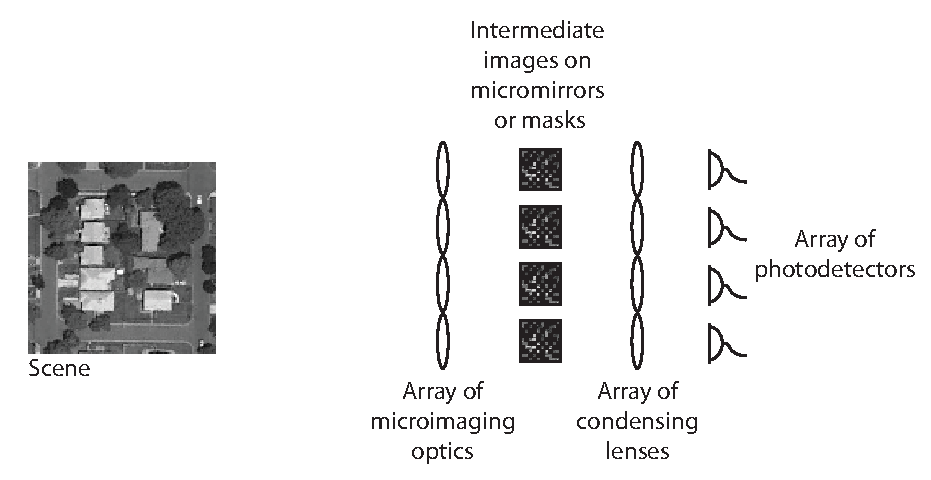
\includegraphics[scale=0.9]{parallelcsimager2}
	\captionof{figure}[The architecture of a hypothetical parallel single pixel camera to capture simultaneous projections.]{An example of a typical parallel optical CS architecture. Capturing $N_m$ simultaneous projections requires using $N_m$ spatial light modulators or masks and $N_m$ detector elements.}
	\label{fig:parallelcsimager2}
\end{figure}




\section{SCOUT Architecture}\label{sec:ScoutArchitecture}

The \gls{scout} uses a volumetric optical components to create all of the measurements simultaneously on a single low resolution \gls{fpa}. Previous prototypes of the \gls{scout} architecture are described in \cite{stenner2010static, rivenson2010single}. A related approach uses optical Radon projections \cite{kashter2012optical}. This approach relies on a several cylindrical lenses to integrate the object plane along a lines on the \gls{fpa}. The number of detector elements is much less than the native dimensionality of the object scene. For a single moving point in the field-of-view two perpendicular Radon projections is enough to compute the change from frame to frame. However, the researchers found heuristically that $4$ cylindrical lens are better for reconstructing the change information for an scene that included up to $10$ moving objects, called movers. 

The \gls{scout} architecture is designed to capture the differences of dynamic scenes while avoiding the hardware scaling issues of the aforementioned \gls{compressive sensing} imaging architectures. The trade-off for the ability to measure parallel projections is the lost flexibility to implement arbitrary projections using an \gls{slm}. However, rather than fully designing the projections themselves, I describe a process for optimizing a parameterized system and analyzing its performance in \Cref{sec:ScoutSimulations}.

The \gls{scout} system takes measurements that are both compressive and multiplexed: The number of measurements must be fewer than the number of scene locations $N_m \ll N$, and each measurement must contain information about many scene locations. In this architecture, the number of measurements is the number of pixels in the \gls{fpa}. Intuitively this means that the system matrix must exhibit a many-to-few mapping from scene locations to \gls{fpa} elements. 

The \gls{scout} architecture is shown in \Cref{fig:scoutArchitecture}. In this architecture the \gls{multiplexing} occurs in the spatial domain using imaging multiple image locations to only a few detector pixels. Instead of using mapping all of the image locations to a single detector, like the single-pixel camera, we create a structured blur. This blur allows the light to be spread to several pixels on the \gls{fpa}. The most straightforward way to achieve a blur is by defocusing the image so that the \gls{psf} is broad, spanning many pixels. Since the \gls{fpa} pixels are large relative to the ultimate reconstruction resolution $N_m \ll N$, this process is compressive. Like any aberration, defocus significantly reduces contrast of high spatial frequencies, so the measurements will poorly conditioned for reconstruction. Therefore, high-frequency structure is imposed atop the blur by coding the optical path with two pseudo-random binary occlusion masks that are placed at different positions between the lens and the sensor. The separation between masks results in spatially varying point-spread function. By using a blur to perform spatial multiplexing and coded apertures to create incoherence in the system matrix, these design elements result in a broad shift-variant \gls{psf}, which is then undersampled.


\begin{figure}
	\includegraphics[scale=1.2]{scoutArchitecture}
	\captionof{figure}[The SCOUT architecture.]{A diagram of the \gls{scout} architecture. A lens projects light through a pair of binary occlusion masks onto a low-resolution sensor which is defocused from the nominal image plane. This creates a spatially multiplexed shift-variant PSF incident on the \gls{fpa}.  }
	\label{fig:scoutArchitecture}
\end{figure}



As with many computational sensing architectures, the forward model is described by 
%
\begin{equation}
	\mb{g} = \mb{H} \mb{f} + \mb{e}
	\label{eq:scoutgHf}
\end{equation}
%
In this equation, the 2-dimensional object scene with $\sqrt{N} \times \sqrt{N}$ elements, is lexicography reordered into a $N \times 1$ column vector, $\mb{f}$. Similarly, the measurement vector $\mb{g}$ is an $N_m \times 1$ vector representing a 2-dimensional measurement with a $\sqrt{N_m} \times \sqrt{N_m}$ matrix which represents the low resolution measurement. The detector noise is represented by the $ N_m \times 1 $ vector $\mb{e}$.

The system matrix $\mb{H}$ is thus $N_m \times N $ matrix, where $N_m \ll N$ in order to the system to be considered compressive. The $n^{th}$ column of $\mb{H}$ describes the \gls{psf} of the $n^{th}$ image element. In other words, each column of the system matrix is the low resolution read-out of the \gls{fpa}. Whereas the $m^{th}$ row of $\mb{H}$ describes the weights of each scene location’s contribution to the $m^{th}$ measurement. In this way, the resulting system matrix $\mb{H}$ demonstrates that the \gls{scout} is a spatially variant optical system and presents a block structure, as seen in the example shown in \Cref{fig:scoutSysResponse}.

\begin{sidewaysfigure}
	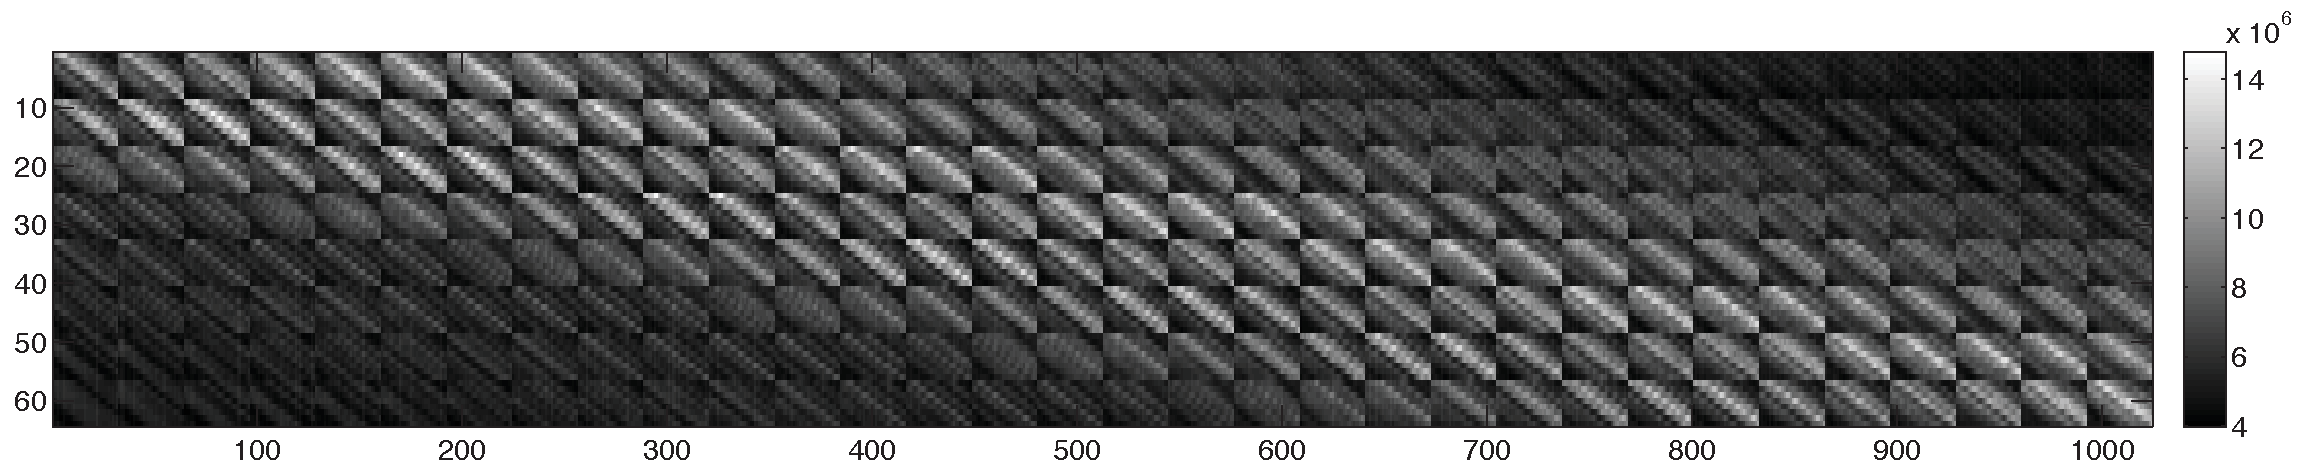
\includegraphics[scale=0.65]{scoutSysResponse}
	\captionof{figure}[An example of the system matrix of the SCOUT.]{An example of an experimentally measured of the system matrix of the \gls{scout} system. The approximate block-Toeplitz structure is clearly evident, as is the deviation from the Bernoulli or Gaussian ensembles typically considered in CS treatments. }
	\label{fig:scoutSysResponse}
\end{sidewaysfigure}


Like any compressive sensing technique, the assumption of a sparse or compressible representation for the signal-of-interest is required. While light from every point in the object scene is recorded, only the differences between successive measurements scenes are processed
%
\begin{equation} 
\begin{split}
	\mb{g}_1 &= \mb{H} \mb{f}_1 + \mb{e}_1 \\
	\mb{g}_2 &= \mb{H} \mb{f}_2 + \mb{e}_2
\end{split}
\end{equation}
%
\begin{equation}
	\mb{g} = \mb{g}_2 - \mb{g}_1 = \mb{H} \ap{ \mb{f}_2 - \mb{f}_1 } + \mb{e}_2 - \mb{e}_1
\end{equation}
%
Where the subscripts represent the readout $k^th$ readout from the \gls{fpa}. Assuming that the background is relatively static between \gls{fpa} exposures, the differences are sparse. Thus the signal-of-interest $\mb{f}$ is sparse. Note that in order to achieve sparsity, there is a trade-off, the system records the noise realization twice. The architecture is modeled as an entirely linear system, so frame differences can be calculated in the measurement basis and subsequently reconstructed in the spatial domain to show dots indicating where an object moved to and from.

Referring back to the diagram of the \gls{scout} architecture shown in \Cref{fig:scoutArchitecture}. A lens of focal length $f$ is focused at infinity and placed some distance $f + d_{im}$ from the sensor. Two binary occlusion masks, $\text{mask}_1$ and $\text{mask}_2$, are placed at distances $dm_1$ and $dm_2$ from the sensor. Masks $\text{mask}_1$ and $\text{mask}_2$, achieve fill factors $\text{ff}_1$ and $\text{ff}_2$ using randomly-patterned occluders of pitch $p_1$ and $p_2$, respectively. The sensor captures images at resolution $ r_x \times r_y = N_m$; adjacent frames are subtracted, and frame differences are reconstructed at some higher resolution $R_x \times R_y = N$ using an $ell_1$ regularized \gls{ls} reconstruction algorithm. In order to enforce the data agreement constraint, the algorithm require knowledge of the $ N_m \times N $ system matrix $\mb{H}$, which is determined through calibration.

Remember that an isomorphic sensor is represented by the identity matrix. In comparison,  in the \gls{scout}, the spatially varying blurred \gls{psf} leads to an approximate block-Toeplitz structure for the system matrix, with approximate Toeplitz structure within individual blocks due to the shifting \gls{psf}. This circulant structure is modified by random variations corresponding to the differing projections created by the two masks. 

As I mentioned in \Cref{chap:Formalism}, random coding has several theoretical properties that make them useful for compressive sensing. There has been some research work to investigate system matrices with Toeplitz and circulant structure \cite{bajwa2007toeplitz, rauhut2009circulant, romberg2009compressive}, however there has been relatively little work published discussing the approximately block-Toeplitz structure that naturally arises in optical systems such as \gls{scout} and theoretical guarantees like the ones force random coding. Two exceptions are \cite{sebert2008toeplitz, liu2008sparsesense}, which provide both theoretical evidence for the viability of CS system matrices with block-Toeplitz structure.

\section{Designing Projections}\label{sec:ScoutSimulations}

\section{Calibration}\label{sec:ScoutCalibrations}

\section{Experimental Results}\label{sec:ScoutExperimentalResults}


\section{Conclusion}

While the \gls{scout} architecture is well-suited for tracking applications, it does have limitations which make it less useful for general imaging applications. Without sparse scene motion, the priors used in reconstruction will lead to incorrect results. Reconstructions only show the locations of moving objects, and the sensing platform must be stationary relative to the scene so that frame differences are sparse. However, more sophisticated techniques could potentially estimate platform motion and use the additional information to reconstruct the entire scene. Despite its limitations, the architecture is well-suited for applications such as fixed-camera wide-area surveillance where bandwidth and data volume are key concerns.


%\bibliographystyle{IEEEtranS}  
%\bibliography{ThesisBib}



